\section{Solving Algorithm}
\label{sec:solving_algorithm}

In order to provide a value for researchers, who upload data to the Captcha service, the system has to label the uploaded images. Thereby, our solving algorithm determines the label based on the given user inputs.\\
In case of text Captchas the algorithm needs at least three users, who solved the Captcha correctly. If three or more suggestions match, the image is marked as solved and labeled accordingly. However, the token is identified as unsolvable if there are six or more proposals but no more than two of them match. This approach is relatively similar to the concept of reCAPTCHA. In a published paper \footnote{http://science.sciencemag.org/content/321/5895/1465.full} it was proven, that three human resolutions are enough to label an image reliably.\\
The method for labeling image Captchas is similar to the one used for texts. The main difference is the fact that the proposals for these are limited to \textit{true} and \textit{false}, if they are suiting the specified task or not. Therefore, the algorithm checks if at least four resolutions match and also declares a token as unsolvable if more than six suggestions are given but failed to produce four that match. It was decided to raise the bar for labeling a picture from three to four, because it is more likely to falsely select an image due to a wrong click.
\begin{figure}[!h]
\centering
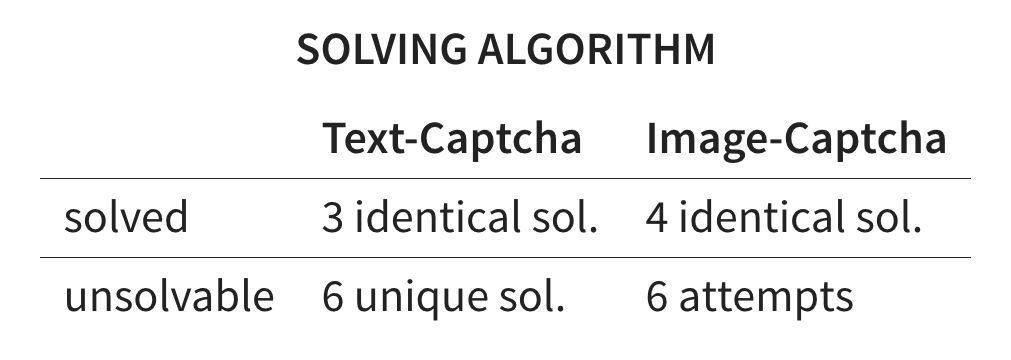
\includegraphics[width=0.8\linewidth]{content/figures/solving_algorithm.png}
\caption{Solving algorithm for text and image Captchas based on user input}
\label{fig:solving_algorithm}
\end{figure}

\clearpage
